%%%%%%%%%%%%%%%%%%%%%%%%%%%%%%%%%%%%%%%%%%%%%%%%%%%%%%%%%%%%%%%%%%%%%%%%%%%%%%%%%%
\begin{frame}[fragile]\frametitle{}
\begin{center}
{\Large Ethereum}
\end{center}
\end{frame}

%%%%%%%%%%%%%%%%%%%%%%%%%%%%%%%%%%%%%%%%%%%%%%%%%%%%%%%%%%%%%%%%%%%%%%%%%%%%%%%%%%
\begin{frame}[fragile]\frametitle{What is Ethereum?}
\begin{itemize}
\item Started by Vitalik Butarin in 2013.
\item Bitcoin is a crypto currency, whereas Ethereum is a platform where people can build apps on top.
\item Its a blockchain which not only allows to store transactions but also programs (Smart Contract) along.
\end{itemize}

\begin{center}
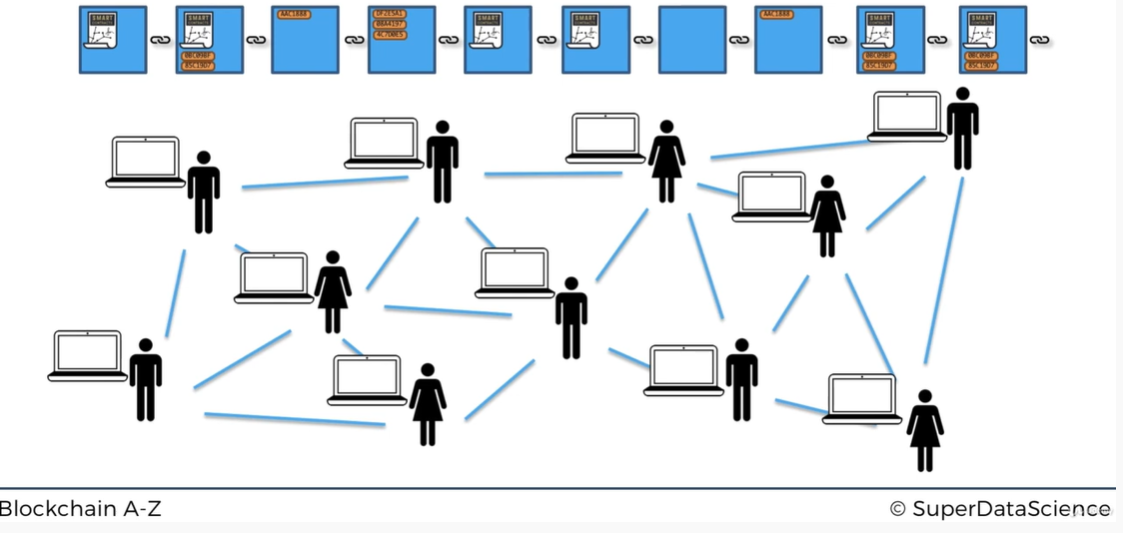
\includegraphics[width=0.6\linewidth,keepaspectratio]{blkchn_20}

{\tiny (Ref: Blockchain A-Z: Learn How To Build Your First Blockchain)}
\end{center}

\end{frame}

%%%%%%%%%%%%%%%%%%%%%%%%%%%%%%%%%%%%%%%%%%%%%%%%%%%%%%%%%%%%%%%%%%%%%%%%%%%%%%%%%%
\begin{frame}[fragile]\frametitle{What is Smart Contract?}
\begin{itemize}
\item A program having rules-code on blockchain nodes.
\item Bitcoin has a script called Bitcoin Script, whereas Ethereum has programming languages Solidity using which Smart Contracts can be programmed.
\item Bitcoin Script is not Turin-Complete, whereas Solidity is.
\item Whats Turin-Complete? meaning, you can code any logic, say, using conditionals, loops, etc. 
\item Bitcoin Script does not have loops, to avoid infinite computation possibilities.
\end{itemize}


\end{frame}


%%%%%%%%%%%%%%%%%%%%%%%%%%%%%%%%%%%%%%%%%%%%%%%%%%%%%%%%%%%%%%%%%%%%%%%%%%%%%%%%%%
\begin{frame}[fragile]\frametitle{So, Ethereum is}
Each node has:
\begin{itemize}
\item History of all Smart Contracts.
\item History of all Transactions.
\item Current state of all Smart Contracts.
\end{itemize}

\begin{center}
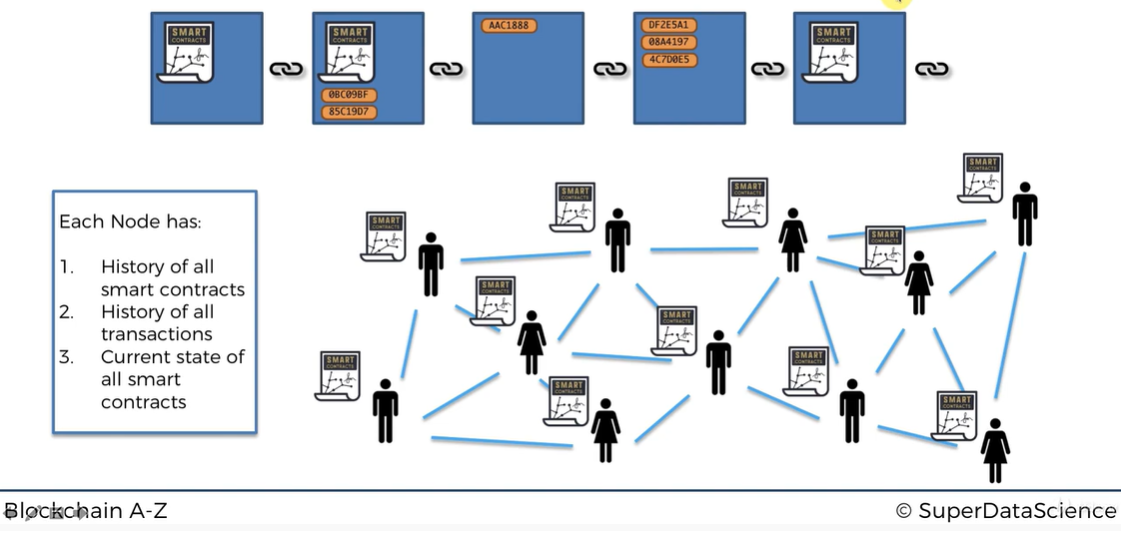
\includegraphics[width=0.6\linewidth,keepaspectratio]{blkchn_22}

{\tiny (Ref: Blockchain A-Z: Learn How To Build Your First Blockchain)}
\end{center}

\end{frame}

%%%%%%%%%%%%%%%%%%%%%%%%%%%%%%%%%%%%%%%%%%%%%%%%%%%%%%%%%%%%%%%%%%%%%%%%%%%%%%%%%%
\begin{frame}[fragile]\frametitle{EVM}
Ethereum Virtual Machine

\begin{itemize}
\item VM running your machine, to run smart contracts.
\item It has no access to outside world on the computer. Secure.
\item Loops are added, but how to curb long computations. Got GAS!!
\item Basically payment to run computation. More computation more money (GAS). 
\item For `addition' operation, say, you need 3 units of GAS.
\item No infinite loop as you will run out of GAS.
\item As Eth as currency is volatile, can predict its price, so instead GAS is purchased first then consumed.
\end{itemize}

\begin{center}
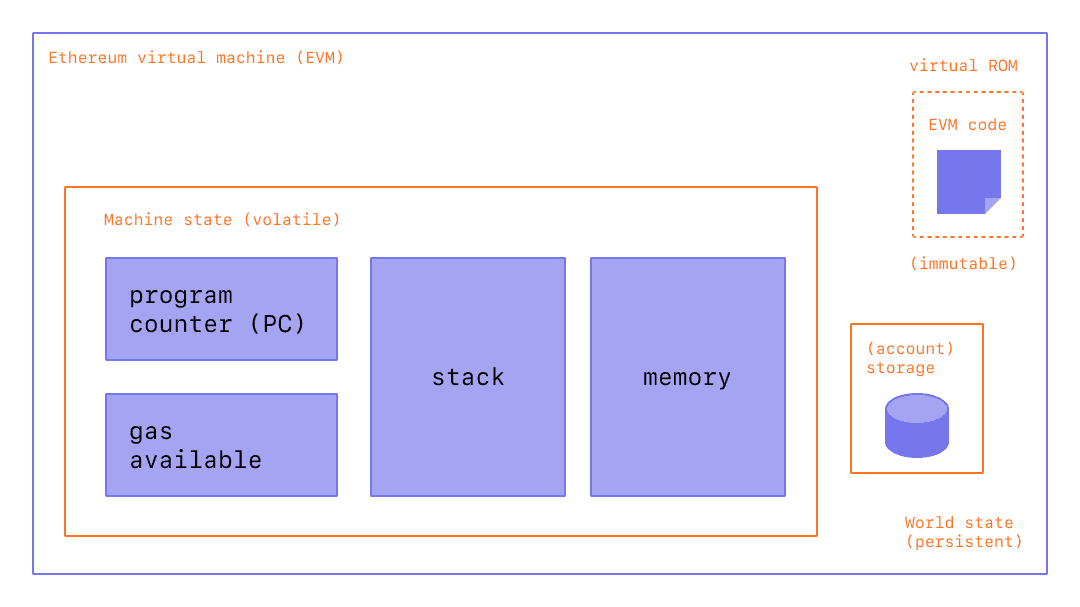
\includegraphics[width=0.5\linewidth,keepaspectratio]{blkchn_23}

{\tiny (Ref: Ethereum Virtual Machine (EVM) | ethereum.org)}
\end{center}

\end{frame}

%%%%%%%%%%%%%%%%%%%%%%%%%%%%%%%%%%%%%%%%%%%%%%%%%%%%%%%%%%%%%%%%%%%%%%%%%%%%%%%%%%
\begin{frame}[fragile]\frametitle{DApps}
Decentralized Apps
\begin{itemize}
\item Front end as app and back-end as Smart Contracts
\item Interface to interact with blockchain, an API
\item Example: Steemit (twitter on blockchain)
\end{itemize}

\begin{center}
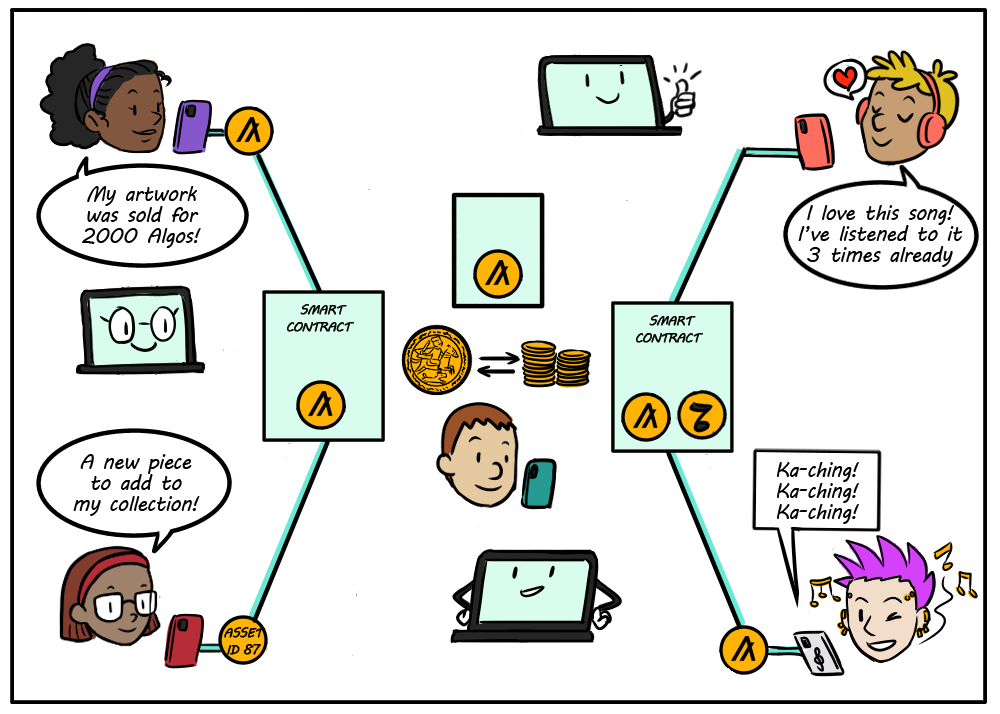
\includegraphics[width=0.6\linewidth,keepaspectratio]{blkchn_21}

{\tiny (Ref: What is a dApp? - Algorand Developer Portal)}
\end{center}

\end{frame}

%%%%%%%%%%%%%%%%%%%%%%%%%%%%%%%%%%%%%%%%%%%%%%%%%%%%%%%%%%%%%%%%%%%%%%%%%%%%%%%%%%
\begin{frame}[fragile]\frametitle{DAQs}
Decentralized Autonomous Organizations

\begin{itemize}
\item Traditional organizations have hierarchies, they follow protocols/processes/work-flows.
\item All these are replaced by Smart Contracts in DAOs. 
\item Basically, not just automated but autonomous.
\item No central decision making, but democratic or decentralized.
\end{itemize}

\begin{center}
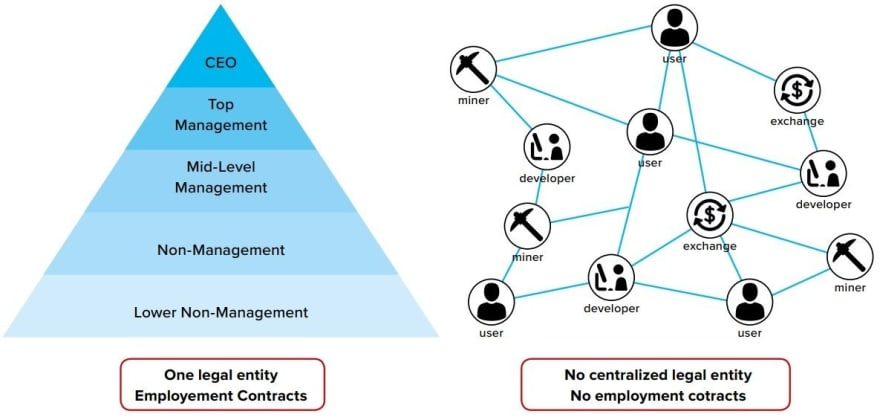
\includegraphics[width=0.6\linewidth,keepaspectratio]{blkchn_24}

{\tiny (Ref: Moralis Academy - Comparing a DAO to a Traditional Organization)}
\end{center}

\end{frame}

%%%%%%%%%%%%%%%%%%%%%%%%%%%%%%%%%%%%%%%%%%%%%%%%%%%%%%%%%%%%%%%%%%%%%%%%%%%%%%%%%%
\begin{frame}[fragile]\frametitle{The DAQ Attack}

\begin{itemize}
\item Started by Vitalik, in 2016, on Ethereum
\item Got funded in May 2016 for \$150M
\item Bug in the Smart Contract code, so there was attack on June 2016 for \$50M
\item There was a breather time before funds moved out, so deliberation happened on if 'Code is Law?'
\item Hard fork, to reverse the transaction. But split happened in Ethereum and new Ethereum Classic (no change advocates) was born.
\item Hacker finally walked away with \$67M in Ethereum Classic.
\end{itemize}


\end{frame}

%%%%%%%%%%%%%%%%%%%%%%%%%%%%%%%%%%%%%%%%%%%%%%%%%%%%%%%%%%%%%%%%%%%%%%%%%%%%%%%%%%
\begin{frame}[fragile]\frametitle{Hard/Soft Fork}

\begin{itemize}
\item Due to DAO attack, Hard (physical split of chain) fork was done on Ethereum, to correct the bug.
\item To increase block size to 8MB, Bitcoin did soft (software split only) fork, called Bitcoin Cash
\item One Hard-fork happened for ASIC resistance and back to GPU, called Bitcoin GOLD
\item Hard fork is not backward compatible, but Soft-fork is. If block size is increased from 1 to 8MB, old block are still within 8MB, anyways, right?
\end{itemize}

\begin{center}
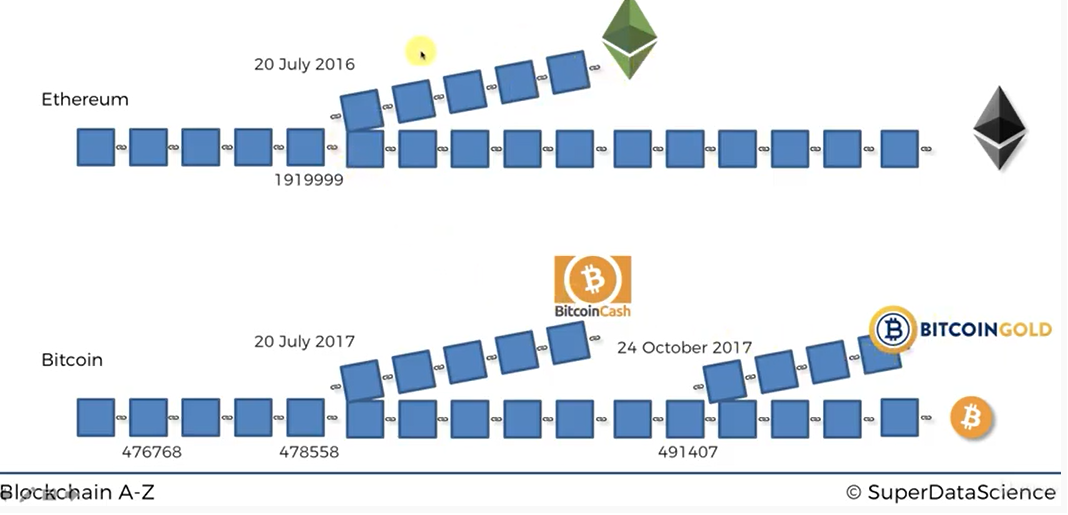
\includegraphics[width=0.6\linewidth,keepaspectratio]{blkchn_25}

{\tiny (Ref: Blockchain A-Z: Learn How To Build Your First Blockchain)}
\end{center}

\end{frame}

%%%%%%%%%%%%%%%%%%%%%%%%%%%%%%%%%%%%%%%%%%%%%%%%%%%%%%%%%%%%%%%%%%%%%%%%%%%%%%%%%%
\begin{frame}[fragile]\frametitle{ICOs}
Initial Coin Offerings

\begin{itemize}
\item Not actually coin but token/idea/functionality offering.
\item IPO (Initial Public Offering): companies offer shares for getting public funds, for the first time.
\item ICOs: give out tokens in exchange of funds/coins. Tokens can be used to buy their products or special permissions.
\end{itemize}

\begin{center}
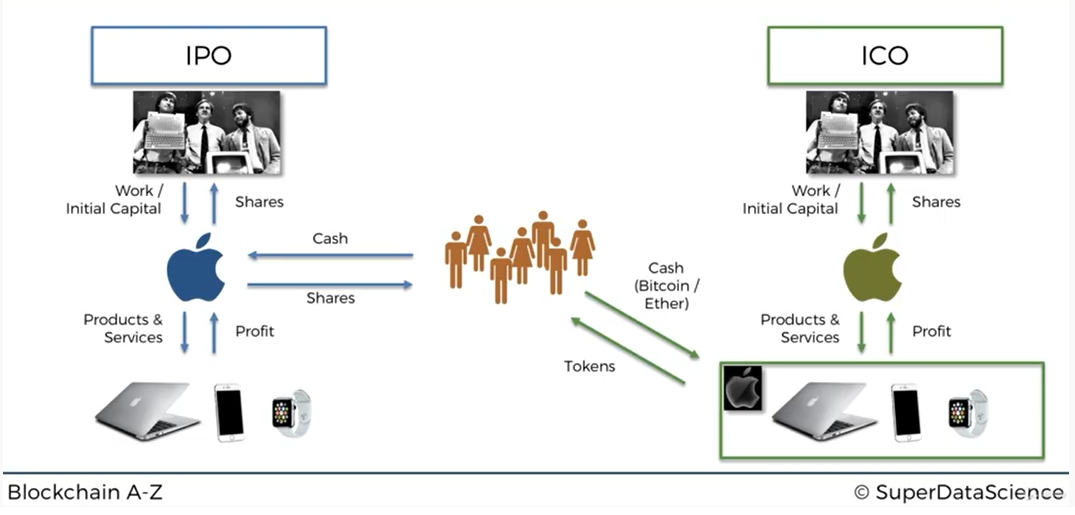
\includegraphics[width=0.6\linewidth,keepaspectratio]{blkchn_26}

{\tiny (Ref: Blockchain A-Z: Learn How To Build Your First Blockchain)}
\end{center}

\end{frame}




